\begin{frame}{Low oxygen pressure}
    \begin{columns}
    
    \column[T]{0.38\textwidth}
    \begin{table}
        \centering
        \begin{tabular}{ |l|l|l|l| }
            \hline
            Argon & \ammonia & \dioxygen & Duration \\
             & & & (hours) \\ 
            \hline
            50 & 0 & 0 & 24 \\
            42 & 0 & 8 & 12 \\
            41 & 1 & 8 & 5 \\
            \hline
            50 & 0 & 0 & 7 \\
            42 & 0 & 8 & 1 \\
            41 & 1 & 8 & 10 \\
            48.5 & 1 & 0.5 & 13 \\
            49 & 1 & 0 & 11 \\
            50 & 0 & 0 & 8 \\
            \hline
            50 & 0 & 0 & 8 \\
            \rowcolor{shadecolor}
            49.5 & 0 & 0.5 & 4 \\
            \hline
        \end{tabular}
        \caption{Gas flow in reactor ($50$ mL/min, $0.3$ bar). In experimental order.}
    \end{table}

    Multiple new peaks appear with only a \textcolor{Important}{very low amount of oxygen} in the reactor.

    \column[T]{0.6\textwidth}
    
        \begin{figure}
        \centering
        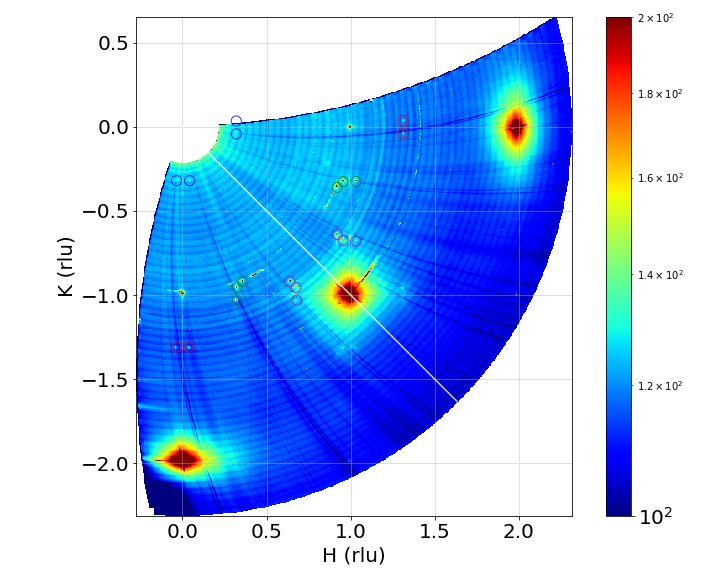
\includegraphics[trim=40 0 40 0, clip, width=0.95\textwidth]{Figures/sxrd_data/maps/Map_hkl_surf_or_2905-2953.png}
        \caption{Reciprocal space map.}
        \label{fig:CondG}
    \end{figure}
        
    \end{columns}

\end{frame}